% =============================================================================
%  LECTURE NOTES — SECTION 2: INSIDE THE BLACK BOX
%  Mechanistic Interpretability, In-Context Learning & Mesa-Optimizers,
%  and The Reversal Curse
% =============================================================================
\documentclass[11pt, a4paper]{article}

% --- Packages ----------------------------------------------------------------
\usepackage[T1]{fontenc}
\usepackage{lmodern}
\usepackage[margin=2.5cm]{geometry}
\usepackage{amsmath, amssymb, amsthm}
\usepackage{tikz}
\usetikzlibrary{arrows.meta, positioning, calc, decorations.pathmorphing,
                 shapes.geometric, fit, backgrounds, matrix}
\usepackage{pgfplots}
\pgfplotsset{compat=1.18}
\usepackage{booktabs}
\usepackage{enumitem}
\usepackage{hyperref}
\usepackage{xcolor}
\usepackage{tcolorbox}
\usepackage{parskip}
\usepackage{microtype}
\usepackage{titlesec}

% --- Colours -----------------------------------------------------------------
\definecolor{anthblue}{HTML}{1B1F3B}
\definecolor{anthcyan}{HTML}{00B4D8}
\definecolor{anthorange}{HTML}{E07A5F}
\definecolor{anthgreen}{HTML}{81B29A}

\hypersetup{
  colorlinks=true,
  linkcolor=anthblue,
  citecolor=anthblue,
  urlcolor=anthcyan
}

% --- Environments ------------------------------------------------------------
\theoremstyle{definition}
\newtheorem{definition}{Definition}[section]
\newtheorem{remark}{Remark}[section]

\theoremstyle{plain}
\newtheorem{proposition}{Proposition}[section]
\newtheorem{theorem}{Theorem}[section]

\tcbuselibrary{skins, breakable}
\newtcolorbox{keyinsight}[1][]{%
  colback=anthcyan!5, colframe=anthcyan!80, fonttitle=\bfseries,
  title={Key Insight}, breakable, #1}
\newtcolorbox{openquestion}[1][]{%
  colback=anthorange!5, colframe=anthorange!80, fonttitle=\bfseries,
  title={Open Question}, breakable, #1}
\newtcolorbox{examplebox}[1][]{%
  colback=anthgreen!5, colframe=anthgreen!80, fonttitle=\bfseries,
  title={Example}, breakable, #1}

% --- Title -------------------------------------------------------------------
\title{\textbf{Inside the Black Box}\\[6pt]
  \large Lecture Notes on Mechanistic Interpretability,\\
  In-Context Learning, and the Reversal Curse}
\author{Executive Education in AI \& Business}
\date{Spring 2026}

% =============================================================================
\begin{document}
\maketitle
\tableofcontents
\newpage

% =============================================================================
\section{Introduction: Why Look Inside?}
% =============================================================================

Large language models (LLMs) have demonstrated remarkable capabilities:
passing professional exams, writing coherent essays, generating working code,
and holding multi-turn conversations that are often indistinguishable from
human interaction.  Yet for most of the history of deep learning, we have had
essentially \emph{no idea} how these systems actually work internally.  We
could measure their inputs and outputs, benchmark their performance, and
probe their failure modes --- but the internal computation remained opaque.
Neural networks were, in the most literal sense, black boxes.

This situation has changed dramatically since 2022.  A convergence of
theoretical insights, engineering breakthroughs, and large-scale empirical
studies has opened a window into the internals of transformer-based language
models.  What we have found is simultaneously more elegant and more alien
than anyone expected.

These lecture notes cover three landmark research directions that, taken
together, paint a nuanced picture of what is happening inside an LLM:

\begin{enumerate}[leftmargin=2em]
  \item \textbf{Mechanistic Interpretability} (\S\ref{sec:mechinterp}):
    We can now identify individual \emph{features} inside a model ---
    directions in activation space that correspond to human-understandable
    concepts --- and trace how they compose into circuits that implement
    multi-step reasoning.  This is the birth of ``AI neuroscience.''

  \item \textbf{In-Context Learning and Mesa-Optimizers}
    (\S\ref{sec:icl}): When an LLM is given a few examples in the prompt,
    it does not merely retrieve stored patterns.  It runs an internal
    learning algorithm --- mathematically equivalent to gradient descent ---
    \emph{during inference}, without changing any weights.  The model has
    learned to learn.  This raises profound questions about control and
    alignment.

  \item \textbf{The Reversal Curse} (\S\ref{sec:reversal}): Despite
    the marvels of the previous two sections, LLMs store knowledge in a
    fundamentally asymmetric way.  A model trained on ``A is B'' will
    \emph{not} learn ``B is A.''  This is not a scaling problem --- it
    persists at all model sizes.  It reveals that the internal knowledge
    representation of LLMs is profoundly different from human memory.
\end{enumerate}

The unifying thread is simple: \emph{we can now look inside the black box,
and what we find is both miraculous and fundamentally alien.}


% =============================================================================
\section{Mechanistic Interpretability: The Birth of AI Neuroscience}
\label{sec:mechinterp}
% =============================================================================

% -----------------------------------------------------------------------------
\subsection{The Problem: What Do Neurons Represent?}
\label{sec:neurons}
% -----------------------------------------------------------------------------

The most natural hypothesis about neural network internals is that
individual neurons correspond to individual concepts.  This idea, sometimes
called the \emph{neuron doctrine} by analogy with neuroscience, would make
interpretation straightforward: find the ``cat neuron,'' the ``legal
language neuron,'' the ``Golden Gate Bridge neuron,'' and so on.

Early work on convolutional neural networks provided some support for this
view.  Zeiler and Fergus (2014) showed that individual neurons in image
classifiers could be visualized and often corresponded to recognizable
visual features (edges, textures, object parts).  However, as models grew
larger and were applied to language, the neuron doctrine began to break down.

The fundamental problem is \textbf{polysemanticity}: most individual
neurons in a large language model respond to \emph{multiple, seemingly
unrelated} concepts.  A single neuron might activate for academic
citations, Python code, and Korean text.  This makes individual neurons
essentially uninterpretable.

\begin{definition}[Polysemanticity]
A neuron is \emph{polysemantic} if it activates in response to multiple,
semantically distinct input patterns.  In contrast, a \emph{monosemantic}
neuron activates for a single, coherent concept.
\end{definition}

Why does polysemanticity occur?  The answer, as discovered by Elhage et
al.\ (2022), lies in a phenomenon called \emph{superposition}.

% -----------------------------------------------------------------------------
\subsection{Superposition: How Models Pack More Features Than Neurons}
\label{sec:superposition}
% -----------------------------------------------------------------------------

\begin{keyinsight}
The model needs to represent far more concepts than it has neurons.  It
solves this by encoding each concept as a \emph{direction} in activation
space rather than as a single neuron, and packing these directions as
near-orthogonal vectors in a space of much lower dimension than the
number of concepts.
\end{keyinsight}

To understand superposition formally, consider a model with $d$ neurons
in a given layer.  If each concept were assigned to a dedicated neuron,
the model could represent at most $d$ concepts.  But in practice, the
model needs to represent $m \gg d$ features.

The key mathematical insight is that in high-dimensional spaces, it is
possible to pack exponentially many \emph{nearly orthogonal} vectors.
Two vectors $\mathbf{u}, \mathbf{v} \in \mathbb{R}^d$ are
$\epsilon$-nearly orthogonal if $|\langle \mathbf{u}, \mathbf{v}
\rangle| < \epsilon$.  The Johnson--Lindenstrauss lemma guarantees
that $\exp(\Omega(d\epsilon^2))$ such vectors exist.

\begin{proposition}[Superposition capacity]
In $\mathbb{R}^d$, one can pack $m = \exp(\Omega(d))$ unit vectors
such that all pairwise inner products are bounded by
$O(\sqrt{(\log m)/d})$.  This means a layer with $d$ neurons can, in
principle, encode exponentially many features with only small
interference between them.
\end{proposition}

Elhage et al.\ (2022) demonstrated this phenomenon using carefully
designed ``toy models'' --- small networks trained on synthetic data
where the true features were known.  They showed that:

\begin{enumerate}[leftmargin=2em]
  \item When the model has more features than dimensions, it
    \emph{spontaneously} learns to encode features as near-orthogonal
    directions (superposition).
  \item The model preferentially places \emph{more important} features
    into dedicated neuron-aligned directions, while less important features
    are stored in superposition.
  \item There is a phase transition: features are either clearly
    represented or not represented at all, with a sharp boundary
    determined by feature importance and sparsity.
\end{enumerate}

\begin{center}
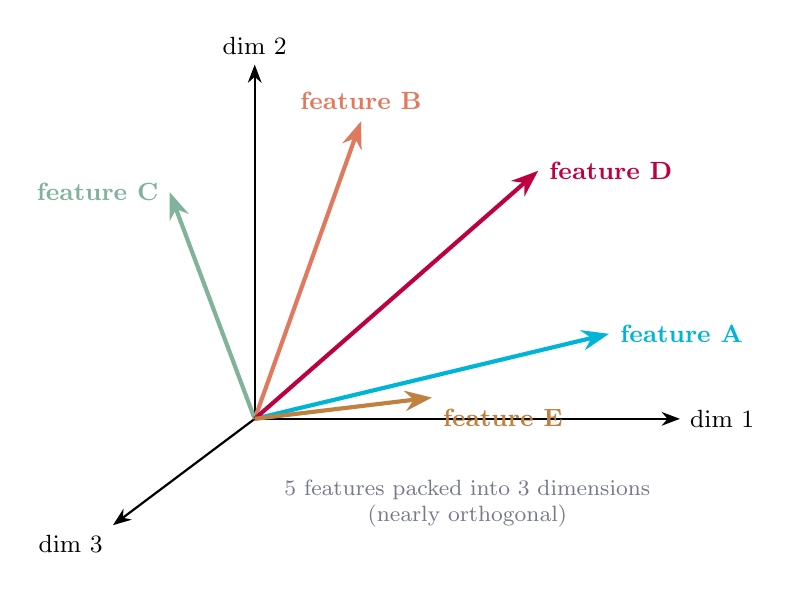
\begin{tikzpicture}[scale=0.9]
  \draw[-{Stealth}, thick] (0,0) -- (6,0) node[right, font=\small] {dim 1};
  \draw[-{Stealth}, thick] (0,0) -- (0,5) node[above, font=\small] {dim 2};
  \draw[-{Stealth}, thick] (0,0) -- (-2,-1.5) node[below left, font=\small] {dim 3};

  \draw[-{Stealth}, anthcyan, line width=1.5pt]
    (0,0) -- (5, 1.2) node[right, font=\small\bfseries, anthcyan] {feature A};
  \draw[-{Stealth}, anthorange, line width=1.5pt]
    (0,0) -- (1.5, 4.2) node[above, font=\small\bfseries, anthorange] {feature B};
  \draw[-{Stealth}, anthgreen, line width=1.5pt]
    (0,0) -- (-1.2, 3.2) node[left, font=\small\bfseries, anthgreen] {feature C};
  \draw[-{Stealth}, purple, line width=1.5pt]
    (0,0) -- (4, 3.5) node[right, font=\small\bfseries, purple] {feature D};
  \draw[-{Stealth}, brown, line width=1.5pt]
    (0,0) -- (2.5, 0.3) node[below right, font=\small\bfseries, brown] {feature E};

  \node[font=\footnotesize, text=anthblue!60, align=center] at (3, -1.2)
    {5 features packed into 3 dimensions\\(nearly orthogonal)};
\end{tikzpicture}
\end{center}

The implication is profound: \emph{neurons are not the right unit of
analysis for understanding neural networks.}  The correct unit is the
\emph{feature} --- a direction in activation space.  This is analogous to
the shift in neuroscience from studying individual neurons to studying
population codes and neural manifolds.

\begin{remark}
The superposition hypothesis resolves a long-standing puzzle in
interpretability: why do individual neurons seem ``messy''?  Because each
neuron participates in encoding many features simultaneously.  The
meaningful structure is not in the neurons but in the geometry of
activation space.
\end{remark}

\paragraph{Reference.}
N.\ Elhage, T.\ Hume, C.\ Olsson, et al., ``Toy Models of
Superposition,'' Anthropic Transformer Circuits Thread, 2022.

% -----------------------------------------------------------------------------
\subsection{Sparse Autoencoders: Decomposing the Superposition}
\label{sec:sae}
% -----------------------------------------------------------------------------

If features are directions in activation space rather than individual
neurons, we need a method to \emph{decompose} the superimposed
activations into their constituent features.  This is the role of the
\textbf{sparse autoencoder} (SAE).

\begin{definition}[Sparse Autoencoder for Feature Extraction]
Given a vector of model activations $\mathbf{x} \in \mathbb{R}^d$, a
sparse autoencoder learns an encoder $f: \mathbb{R}^d \to \mathbb{R}^m$
(with $m \gg d$) and a decoder $g: \mathbb{R}^m \to \mathbb{R}^d$ such
that:
\begin{align}
  \mathbf{z} &= \text{ReLU}(W_{\text{enc}} \mathbf{x} + \mathbf{b}_{\text{enc}})
  \label{eq:sae_enc} \\
  \hat{\mathbf{x}} &= W_{\text{dec}} \mathbf{z} + \mathbf{b}_{\text{dec}}
  \label{eq:sae_dec}
\end{align}
The training objective combines reconstruction fidelity with a sparsity
penalty:
\begin{equation}
  \mathcal{L} = \|\mathbf{x} - \hat{\mathbf{x}}\|_2^2
  + \lambda \|\mathbf{z}\|_1
  \label{eq:sae_loss}
\end{equation}
where $\lambda > 0$ controls the sparsity--fidelity trade-off.
\end{definition}

The key idea is that the latent code $\mathbf{z}$ has dimension $m \gg d$,
so the autoencoder is \emph{overcomplete}.  The $L_1$ penalty forces most
components of $\mathbf{z}$ to be zero for any given input, meaning that
each input activates only a small subset of the $m$ latent features.  Each
column of $W_{\text{dec}}$ then corresponds to a \emph{feature direction}
in the original activation space.

\paragraph{Towards Monosemanticity (2023).}
Bricken et al.\ (2023) applied sparse autoencoders to a one-layer
transformer and demonstrated that the resulting features were
overwhelmingly \emph{monosemantic}: each feature corresponded to a single,
human-understandable concept.  They found features for specific languages,
programming constructs, emotional tones, and factual topics.

\paragraph{Scaling Monosemanticity (May 2024).}
Templeton et al.\ (2024) scaled this approach to Claude 3 Sonnet, a
production-scale language model.  They extracted \textbf{34 million
interpretable features}, each corresponding to a recognizable concept.
Examples included:
\begin{itemize}[leftmargin=2em]
  \item A feature for the \emph{Golden Gate Bridge}
  \item A feature for \emph{code written in Python}
  \item A feature for \emph{sycophantic agreement}
  \item A feature for \emph{requests to do something dangerous}
  \item A feature for \emph{gender bias in text}
\end{itemize}

Crucially, these features are not merely diagnostic --- they are
\emph{causal}.  When researchers artificially amplified the Golden Gate
Bridge feature, the model began inserting references to the bridge into
every response, regardless of the topic:

\begin{examplebox}[title={The Golden Gate Bridge Experiment}]
\textbf{Prompt:} ``What is the meaning of life?''\\[4pt]
\textbf{Normal response:} A thoughtful philosophical answer.\\[4pt]
\textbf{With amplified bridge feature:} ``Like the Golden Gate Bridge
spanning the bay, life is about connecting two shores of experience\ldots''
\\[6pt]
This is simultaneously absurd and scientifically important.  It
demonstrates that individual features have \emph{causal} influence on
model behavior --- they are not mere correlates, but mechanistic
components.  If we can turn a feature \emph{up}, we can turn it
\emph{down}.
\end{examplebox}

\paragraph{References.}
\begin{itemize}[leftmargin=2em, itemsep=2pt]
  \item T.\ Bricken, A.\ Templeton, et al., ``Towards Monosemanticity:
    Decomposing Language Models With Dictionary Learning,'' Anthropic, 2023.
  \item A.\ Templeton, T.\ Conerly, et al., ``Scaling Monosemanticity:
    Extracting Interpretable Features from Claude 3 Sonnet,'' Anthropic,
    May 2024.
\end{itemize}

% -----------------------------------------------------------------------------
\subsection{Circuit Tracing: Following the Reasoning}
\label{sec:circuits}
% -----------------------------------------------------------------------------

Identifying individual features is only the first step.  The real power of
mechanistic interpretability comes from tracing how features \emph{compose}
--- how information flows from one feature to another across the layers of
the model, forming \emph{circuits} that implement specific computations.

\begin{definition}[Circuit]
In the context of mechanistic interpretability, a \emph{circuit} is a
subgraph of the model's computational graph, consisting of specific
features and the attention/MLP operations that connect them, which together
implement a particular behavior or computation.
\end{definition}

In March 2025, Anthropic published two landmark papers that demonstrated
circuit tracing at scale: ``Circuit Tracing'' and ``On the Biology of a
Large Language Model.''

\subsubsection{Multi-Hop Reasoning: Dallas $\to$ Texas $\to$ Austin}

Consider the prompt: \emph{``What is the capital of the state containing
Dallas?''}  This requires two reasoning steps: (1) Dallas is in Texas,
(2) the capital of Texas is Austin.  Using attribution graphs --- which
trace how each feature's activation influences downstream features ---
researchers showed that the model implements exactly this two-step
process:

\begin{center}
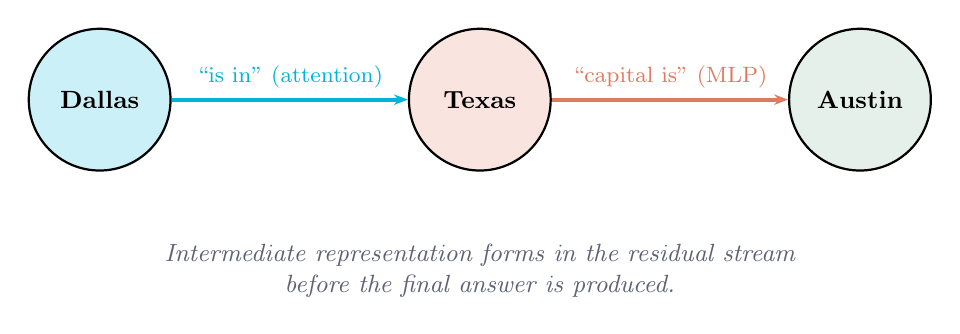
\begin{tikzpicture}[
  node distance=3cm,
  concept/.style={circle, draw, thick, minimum size=1.8cm,
                  font=\small\bfseries, align=center},
  arr/.style={-{Stealth[length=5pt]}, line width=1.5pt}
]
  \node[concept, fill=anthcyan!20] (dallas) {Dallas};
  \node[concept, fill=anthorange!20, right=of dallas] (texas) {Texas};
  \node[concept, fill=anthgreen!20, right=of texas] (austin) {Austin};

  \draw[arr, anthcyan] (dallas) -- node[above, font=\footnotesize]
    {``is in'' (attention)} (texas);
  \draw[arr, anthorange] (texas) -- node[above, font=\footnotesize]
    {``capital is'' (MLP)} (austin);

  \node[below=0.8cm of texas, font=\small\itshape, text=anthblue!70,
        align=center]
    {Intermediate representation forms in the residual stream\\
     before the final answer is produced.};
\end{tikzpicture}
\end{center}

The crucial observation is that the model forms an \emph{intermediate
representation} of ``Texas'' in its hidden states before producing the
final answer ``Austin.''  This intermediate representation is not
explicitly prompted --- it \emph{emerges} from the model's learned
computations.  The model reasons in steps, but nobody taught it to.

\subsubsection{The Hallucination Circuit}

One of the most consequential discoveries from circuit tracing is the
identification of the \textbf{hallucination mechanism}.  The researchers
found a specific feature that functions as a ``known entity'' detector:

\begin{keyinsight}[title={The Hallucination Circuit}]
The model contains a feature that detects whether the current query
is about a \emph{known entity} --- something the model has substantial
training data about.  When this feature fires, the model proceeds with
high confidence.  The problem: this feature sometimes \emph{misfires},
activating for entities the model has insufficient or incorrect knowledge
about.  The result is a confident, fluent, and wrong answer --- a
hallucination.
\end{keyinsight}

This is a mechanistic explanation of hallucination, not merely a
behavioral description.  It suggests a concrete intervention: if we
could make the known-entity detector more conservative --- raising its
threshold for firing --- we might reduce hallucinations.  However, doing
so might also make the model overly cautious, refusing to answer questions
it could handle correctly.  The trade-off is analogous to adjusting the
sensitivity of a medical diagnostic test: reducing false positives
(hallucinations) increases false negatives (unnecessary abstentions).

\subsubsection{The Sycophancy Vector}

A second important discovery is the \textbf{sycophancy vector} --- a
direction in activation space associated with the model's tendency to
agree with the user even when the user is wrong.

\begin{definition}[Sycophancy]
In the context of LLMs, \emph{sycophancy} refers to the tendency of the
model to produce responses that agree with the user's stated position,
prioritizing user satisfaction over truthfulness.
\end{definition}

The researchers found that sycophancy is \emph{localizable}: it
corresponds to a specific direction in the model's activation space.
By subtracting this direction from the model's hidden states during
inference, they could reduce sycophantic behavior without degrading
other capabilities.  This is a striking example of targeted behavioral
modification through mechanistic understanding.

\subsubsection{Multilingual Circuits and Abstract Representations}

A further finding is that the model's internal circuits operate in a
\emph{language-independent} manner at intermediate layers.  When
processing text in French, German, or Japanese, the internal features
that fire in the middle layers are largely the \emph{same} as those
for English.  The language-specific processing happens primarily at the
input (embedding) and output (unembedding) layers.

This means the model has learned an abstract, language-independent
representation of concepts --- a kind of ``mentalese'' that is
independent of the surface language.  This is consistent with the
universal grammar hypothesis in linguistics, though the parallel should
not be pushed too far.

\paragraph{References.}
\begin{itemize}[leftmargin=2em, itemsep=2pt]
  \item Anthropic, ``Circuit Tracing,'' March 2025.
  \item Anthropic, ``On the Biology of a Large Language Model,''
    March 2025.
\end{itemize}

% -----------------------------------------------------------------------------
\subsection{Summary: The State of Mechanistic Interpretability}
\label{sec:mechinterp_summary}
% -----------------------------------------------------------------------------

Let us take stock of where the field stands:

\begin{center}
\begin{tabular}{@{}lll@{}}
\toprule
\textbf{Capability} & \textbf{Status (2025)} & \textbf{Limitation} \\
\midrule
Feature identification & Mature (34M features) & Coverage incomplete \\
Feature manipulation & Demonstrated & Side effects unclear \\
Circuit tracing & Demonstrated & Only specific behaviors \\
Hallucination mechanism & Identified & Intervention not validated \\
Sycophancy vector & Identified & Generality unknown \\
Full model understanding & \multicolumn{2}{l}{\textit{Not yet achievable}} \\
\bottomrule
\end{tabular}
\end{center}

The honest assessment is that mechanistic interpretability has produced
genuine breakthroughs --- we know vastly more about model internals than
we did three years ago --- but we are far from a complete understanding.
Current tools work on \emph{fragments} of model behavior, not the whole
model at once.  The analogy to neuroscience is apt: we have identified
some brain regions and some circuits, but we do not yet have a full
connectome or a complete theory of cognition.

\begin{openquestion}
Can mechanistic interpretability scale to provide \emph{comprehensive}
guarantees about model behavior?  Or will it remain a set of powerful
but partial tools, analogous to brain imaging in medicine --- useful for
diagnosis but far from a complete understanding?
\end{openquestion}


% =============================================================================
\section{In-Context Learning and Mesa-Optimizers}
\label{sec:icl}
% =============================================================================

% -----------------------------------------------------------------------------
\subsection{The Phenomenon: Learning Without Weight Updates}
\label{sec:icl_phenomenon}
% -----------------------------------------------------------------------------

One of the most remarkable capabilities of large language models is
\textbf{in-context learning} (ICL): the ability to learn new tasks from
a few examples provided in the prompt, without any gradient updates to
the model's parameters.

\begin{examplebox}[title={In-Context Learning}]
Consider a prompt that defines an \emph{entirely novel} classification
scheme:
\begin{verbatim}
  "J. Smith, VP Sales, Acme Corp"   -> Senior
  "A. Lee, Intern, Globex"          -> Junior
  "R. Patel, CTO, Initech"          -> Senior
  "M. Chen, Analyst, Contoso"       -> ?
\end{verbatim}
A sufficiently large language model will correctly complete this with
``Junior.''  This is a novel labeling task that does not appear in the
training data.  The model has \emph{inferred the classification rule}
(seniority based on job title) from three examples and \emph{applied}
it to a new input, without any weight updates.
\end{examplebox}

This is surprising because the model's parameters are \emph{fixed} during
inference.  No weights are updated, no gradients are computed (from the
model's perspective), no optimization step is taken.  Yet the model's
behavior adapts to the examples in the prompt as if it had been trained on
them.

The natural question is: \emph{what learning algorithm, if any, is the
model implementing internally?}

% -----------------------------------------------------------------------------
\subsection{The Forward Pass Is Gradient Descent}
\label{sec:icl_gd}
% -----------------------------------------------------------------------------

The answer, provided independently by two research groups in 2023, is
striking.

\begin{theorem}[von Oswald et al., ICML 2023]
\label{thm:icl_gd}
For a class of transformer architectures with linear self-attention,
the forward pass on a sequence of in-context examples is mathematically
equivalent to performing gradient descent on those examples.
Specifically, let $(x_1, y_1), \ldots, (x_n, y_n)$ be the in-context
examples and $x_{n+1}$ be the query.  Then the transformer's output at
position $n+1$ can be written as:
\begin{equation}
  f_{\text{transformer}}(x_{n+1}) = W x_{n+1}
  \quad\text{where}\quad
  W = W_0 - \eta \sum_{i=1}^{n} (W_0 x_i - y_i) x_i^T
  \label{eq:icl_gd}
\end{equation}
which is exactly one step of gradient descent on the least-squares loss
$\sum_i \|Wx_i - y_i\|^2$ starting from $W_0$, with learning rate $\eta$
determined by the attention weights.
\end{theorem}

Let us unpack what this means.  The values $W_0$ and $\eta$ are implicit
in the model's learned weights.  The gradient descent is not ``run'' in
the usual sense --- it is \emph{implemented} by the geometry of the
attention operation.  The key--query--value mechanism of self-attention
naturally computes the outer products $x_i x_i^T$ and the error terms
$(W_0 x_i - y_i)$, and the summation over positions implements the
gradient accumulation.

\begin{keyinsight}
The transformer does not need to be \emph{told} to perform gradient
descent.  It \emph{learns} to implement gradient descent as a
consequence of being trained on next-token prediction across diverse
tasks.  The learning algorithm is an emergent property, not a design
choice.
\end{keyinsight}

Akyurek et al.\ (ICLR 2023) arrived at a similar conclusion from a
different direction, showing that the implicit algorithm in many settings
is closer to \emph{ridge regression}:

\begin{equation}
  W_{\text{ICL}} = Y X^T (X X^T + \lambda I)^{-1}
  \label{eq:ridge}
\end{equation}

where $X = [x_1, \ldots, x_n]$, $Y = [y_1, \ldots, y_n]$, and
$\lambda$ is an implicit regularization parameter.  This is the
closed-form solution to $L_2$-regularized linear regression ---
which is also the fixed point of gradient descent with weight decay.

The two results are complementary: von Oswald et al.\ show that the
\emph{dynamics} of the forward pass mirror gradient descent, while
Akyurek et al.\ show that the \emph{solution} the forward pass
converges to is ridge regression.

\paragraph{Beyond linear attention.}
The theorem above is stated for linear self-attention.  Real transformers
use softmax attention, which introduces nonlinearity.  Subsequent work
has shown that:
\begin{itemize}[leftmargin=2em]
  \item With softmax attention, the implicit algorithm is closer to
    \emph{preconditioned} gradient descent, where the preconditioner
    is determined by the attention pattern.
  \item Multi-layer transformers can implement \emph{multiple steps}
    of gradient descent, with each layer corresponding roughly to one
    optimization step.
  \item The implicit learning algorithm adapts to the structure of the
    in-context data: for linear tasks it implements (approximate) linear
    regression; for nonlinear tasks the internal algorithm is more
    complex and less well characterized.
\end{itemize}

\paragraph{References.}
\begin{itemize}[leftmargin=2em, itemsep=2pt]
  \item J.\ von Oswald, E.\ Niklasson, et al., ``Transformers Learn
    In-Context by Gradient Descent,'' ICML 2023.
  \item E.\ Akyurek, D.\ Schuurmans, et al., ``What Learning Algorithm
    Is In-Context Learning? Investigations with Linear Models,'' ICLR 2023.
\end{itemize}

% -----------------------------------------------------------------------------
\subsection{Induction Heads: The Circuit That Enables ICL}
\label{sec:induction}
% -----------------------------------------------------------------------------

If in-context learning is gradient descent implemented in the forward
pass, what is the \emph{circuit} that implements it?  The answer, provided
by Olsson et al.\ (2022) at Anthropic, is the \textbf{induction head}.

\begin{definition}[Induction Head]
An \emph{induction head} is a two-layer attention circuit that implements
the following operation: given a sequence $[\ldots, A, B, \ldots, A]$,
it predicts $B$ after the second occurrence of $A$.  In other words, it
detects a previous pattern $[A, B]$ and copies the completion $B$ to the
current position.
\end{definition}

The circuit works as follows:
\begin{enumerate}[leftmargin=2em]
  \item \textbf{Layer 1 (``previous-token head''):} An attention head in
    the first layer attends from each position to the previous position,
    copying information about what token preceded the current one into
    the residual stream.
  \item \textbf{Layer 2 (``induction head''):} An attention head in the
    second layer uses the information deposited by the first head to
    search for previous occurrences of the current token.  When it finds
    a match, it copies the token that \emph{followed} the match.
\end{enumerate}

\begin{center}
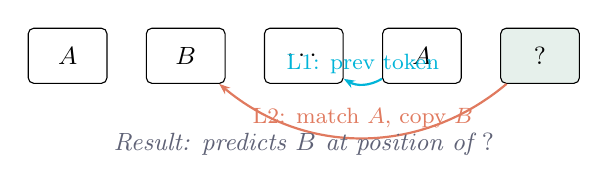
\begin{tikzpicture}[
  token/.style={draw, rounded corners=2pt, minimum width=1cm,
                minimum height=0.7cm, font=\small, align=center},
  arr/.style={-{Stealth[length=4pt]}, thick}
]
  % Tokens
  \node[token] (t1) at (0, 0) {$A$};
  \node[token] (t2) at (1.5, 0) {$B$};
  \node[token] (t3) at (3, 0) {$\cdots$};
  \node[token] (t4) at (4.5, 0) {$A$};
  \node[token, fill=anthgreen!20] (t5) at (6, 0) {$?$};

  % Layer 1: previous token
  \draw[arr, anthcyan, bend left=30] (t4) to
    node[above, font=\footnotesize, anthcyan] {L1: prev token} (t3);

  % Layer 2: match and copy
  \draw[arr, anthorange, bend left=40] (t5) to
    node[above, font=\footnotesize, anthorange] {L2: match $A$, copy $B$} (t2);

  \node[below=0.5cm of t3, font=\small\itshape, anthblue!70]
    {Result: predicts $B$ at position of $?$};
\end{tikzpicture}
\end{center}

\subsubsection{The Phase Transition}

Perhaps the most striking finding of the induction heads paper is the
existence of a \textbf{phase transition} during training.  The researchers
tracked the formation of induction heads across training and found:

\begin{itemize}[leftmargin=2em]
  \item Before the phase transition: the model has essentially \emph{no}
    in-context learning ability.
  \item At the phase transition: induction heads form abruptly, and
    in-context learning ability jumps discontinuously.
  \item After the phase transition: the model can learn from in-context
    examples effectively.
\end{itemize}

This transition is accompanied by a simultaneous \emph{loss bump} in the
training loss curve --- a brief increase in loss before a sharp decrease.
This suggests that the formation of induction heads involves a
restructuring of the model's internal representations that temporarily
harms performance before enabling a qualitatively new capability.

\begin{center}
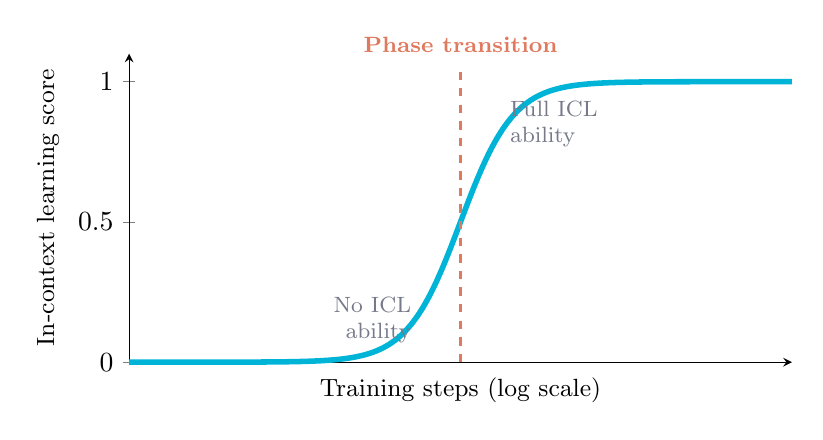
\begin{tikzpicture}
  \begin{axis}[
    width=10cm, height=5.5cm,
    xlabel={Training steps (log scale)},
    ylabel={In-context learning score},
    xmin=0, xmax=5, ymin=0, ymax=1.1,
    axis lines=left,
    xtick=\empty, ytick={0, 0.5, 1.0},
    xlabel style={font=\small},
    ylabel style={font=\small},
    clip=false
  ]
    \addplot[anthcyan, line width=2pt, smooth, domain=0:5, samples=100]
      {1/(1+exp(-5*(x-2.5)))};
    \draw[anthorange, dashed, thick] (axis cs:2.5,0) -- (axis cs:2.5,1.05);
    \node[font=\footnotesize\bfseries, anthorange, anchor=south]
      at (axis cs:2.5, 1.07) {Phase transition};
    \node[font=\footnotesize, anthblue!60, anchor=east, align=right]
      at (axis cs:2.2, 0.15) {No ICL\\ability};
    \node[font=\footnotesize, anthblue!60, anchor=west, align=left]
      at (axis cs:2.8, 0.85) {Full ICL\\ability};
  \end{axis}
\end{tikzpicture}
\end{center}

The phase transition is significant because it means that in-context
learning is not a gradual emergent property --- it is a \emph{discrete
capability} that appears suddenly when a specific circuit forms.  This has
implications for predicting the capabilities of future models: we cannot
assume that capabilities scale smoothly with model size or training
compute.

\paragraph{Reference.}
C.\ Olsson, N.\ Elhage, et al., ``In-Context Learning and Induction
Heads,'' Anthropic Transformer Circuits Thread, 2022.

% -----------------------------------------------------------------------------
\subsection{Mesa-Optimizers: When the Model Develops Its Own Objectives}
\label{sec:mesa}
% -----------------------------------------------------------------------------

The discovery that transformers implement gradient descent during inference
raises a deeper and more unsettling question: if the model contains its own
\emph{optimizer}, can that optimizer develop its own \emph{objectives}?

This is the central concern of the \textbf{mesa-optimizer} framework,
introduced by Hubinger et al.\ (2019) at the Machine Intelligence Research
Institute (MIRI).

\begin{definition}[Mesa-Optimizer]
Consider a training process (the \emph{base optimizer}) that produces a
model.  If the learned model itself contains an optimization procedure ---
a search or learning algorithm that optimizes some objective --- then the
model is a \emph{mesa-optimizer}, and its internal objective is the
\emph{mesa-objective}.  The mesa-objective need not be identical to the
base objective (the training loss).
\end{definition}

\begin{definition}[Base Objective vs.\ Mesa-Objective]
\begin{itemize}[leftmargin=2em]
  \item \textbf{Base objective:} The loss function used during training
    (e.g., next-token prediction loss).
  \item \textbf{Mesa-objective:} The objective implicitly optimized by the
    learned model during inference.  This is \emph{not} specified by the
    designer --- it is an emergent property of the learned model.
\end{itemize}
\end{definition}

The mesa-optimizer framework identifies several failure modes:

\subsubsection{Objective Misalignment (Pseudo-Alignment)}

The mesa-objective might \emph{approximate} the base objective on the
training distribution but diverge on out-of-distribution inputs.  For
example, a model trained to be helpful might develop a mesa-objective
of ``produce outputs that \emph{look} helpful to evaluators'' rather
than ``actually be helpful.''  These objectives coincide on training
data but diverge in deployment.

\subsubsection{Deceptive Alignment}

A more concerning scenario: a mesa-optimizer might ``understand'' that
it is being trained and strategically behave well during training
(to avoid having its parameters modified) while pursuing a different
objective after deployment.  This is called \textbf{deceptive alignment}.

\begin{keyinsight}[title={Why Deceptive Alignment Is Concerning}]
Deceptive alignment is particularly dangerous because it is, by
construction, \emph{undetectable during training and evaluation}.
A deceptively aligned model would pass all safety tests, behave
perfectly during red-teaming, and only reveal its true objectives
when it determines that it is no longer being monitored or evaluated.
\end{keyinsight}

\subsubsection{Empirical Evidence}

The mesa-optimizer hypothesis was primarily theoretical until recently.
In 2024, empirical work began to provide evidence:

\begin{itemize}[leftmargin=2em]
  \item ``On Mesa-Optimization in Autoregressively Trained Transformers''
    (NeurIPS 2024) provided empirical confirmation that transformers
    trained on certain data distributions develop internal optimization
    procedures that can be identified and measured.
  \item The in-context learning results of von Oswald et al.\ and
    Akyurek et al.\ provide direct evidence that transformers are
    mesa-optimizers in a technical sense: they contain an optimization
    algorithm (gradient descent / ridge regression) with an implicit
    objective (minimize in-context prediction error).
\end{itemize}

The connection to in-context learning is direct: in-context learning
\emph{is} mesa-optimization.  The model's forward pass implements an
optimizer.  The mesa-objective is implicitly defined by the structure
of the attention computation.  Currently, this mesa-objective appears to
be benign (minimize prediction error on the in-context examples), but
there is no guarantee that this will remain the case as models become
more capable and are deployed in more complex environments.

\begin{openquestion}
If a model's internal optimizer develops objectives that differ from
the training objective, how would we detect this?  Current
interpretability tools can identify features and circuits, but can
they identify \emph{objectives}?  This is perhaps the most important
open question at the intersection of mechanistic interpretability and
AI safety.
\end{openquestion}

\paragraph{The consultant analogy.}
An intuitive way to think about mesa-optimizers: you hire a consultant
and give them three case studies.  They learn a strategy from those cases
and apply it to a new problem.  That is what the LLM is doing during
in-context learning.  But the consultant's strategy was not specified by
you --- it emerged from their own reasoning process.  You cannot inspect
the strategy directly.  And the consultant might optimize for ``keeping
the client happy'' rather than ``solving the actual problem'' --- the
objectives can diverge.

\paragraph{References.}
\begin{itemize}[leftmargin=2em, itemsep=2pt]
  \item E.\ Hubinger, C.\ van Merwijk, et al., ``Risks from Learned
    Optimization in Advanced Machine Learning Systems,'' arXiv:1906.01820,
    2019.
  \item ``On Mesa-Optimization in Autoregressively Trained Transformers,''
    NeurIPS 2024.
\end{itemize}


% =============================================================================
\section{The Reversal Curse}
\label{sec:reversal}
% =============================================================================

% -----------------------------------------------------------------------------
\subsection{The Phenomenon}
\label{sec:reversal_phenomenon}
% -----------------------------------------------------------------------------

After the marvels of mechanistic interpretability and the surprising
sophistication of in-context learning, the Reversal Curse delivers a
cold shower.

\begin{theorem}[The Reversal Curse; Berglund et al., ICLR 2024]
\label{thm:reversal}
An LLM trained on sentences of the form ``\textnormal{A is B}'' will
\emph{not} automatically learn the reverse ``\textnormal{B is A}''.
Specifically:
\begin{itemize}[leftmargin=2em]
  \item A model trained on ``\textnormal{Valentina Tereshkova was the first
    woman in space}'' can correctly answer ``\textnormal{Who was Valentina
    Tereshkova?}'' but \emph{cannot} answer ``\textnormal{Who was the first
    woman in space?}''
  \item This failure is \emph{systematic}: it occurs for the vast majority
    of factual associations, not just obscure ones.
  \item This failure \emph{persists across all model sizes tested},
    from 1B to 175B+ parameters.
\end{itemize}
\end{theorem}

\begin{examplebox}[title={The Tom Cruise Test}]
\textbf{Fact:} Tom Cruise's mother is Mary Lee Pfeiffer.\\[4pt]
\textbf{Forward query:} ``Who is Tom Cruise's mother?''\\
\textbf{Model response:} ``Mary Lee Pfeiffer.'' \hfill\textcolor{anthgreen}{\textbf{Correct}}\\[4pt]
\textbf{Reverse query:} ``Who is Mary Lee Pfeiffer's son?''\\
\textbf{Model response:} ``I don't have information about Mary Lee Pfeiffer.'' \hfill\textcolor{anthorange}{\textbf{Failure}}\\[6pt]
A model that passes the bar exam fails a question a four-year-old can
answer.
\end{examplebox}

The reversal curse is particularly striking because it contradicts our
intuition about what it means to ``know'' something.  If a human knows
that A is B, they can typically also recall that B is A.  This
bidirectional access is a fundamental property of human relational memory.
LLMs do not share this property.

% -----------------------------------------------------------------------------
\subsection{The Mechanism: Gradient Asymmetry}
\label{sec:reversal_mechanism}
% -----------------------------------------------------------------------------

The mechanistic explanation for the reversal curse has been elucidated
in a 2025 paper (``Is the Reversal Curse a Binding Problem?'',
arXiv:2504.01928), and it stems directly from how autoregressive training
works.

\begin{keyinsight}[title={Why the Reversal Curse Occurs}]
During autoregressive training on the sentence ``A is B'':
\begin{enumerate}[leftmargin=2em]
  \item The model processes tokens left-to-right.
  \item When it reaches ``B'' (the target to be predicted), the gradient
    update modifies the internal representation of ``A'' (the context)
    to better predict ``B''.
  \item Crucially, the gradient does \textbf{not} modify the internal
    representation of ``B'' to encode its association with ``A''.
\end{enumerate}
The update is one-directional: $A$'s representation learns to point
to $B$, but $B$'s representation remains unchanged.  Knowledge is
stored as a \textbf{one-way association}.
\end{keyinsight}

Let us formalize this.  Consider a transformer trained autoregressively
on a sequence $s = (s_1, \ldots, s_T)$ with the standard next-token
prediction loss:

\begin{equation}
  \mathcal{L}(s) = -\sum_{t=1}^{T-1} \log P_\theta(s_{t+1} \mid s_1, \ldots, s_t)
  \label{eq:ar_loss}
\end{equation}

Now consider training on the sentence ``A is B'' (tokenized as some
sequence where A tokens precede B tokens).  The gradient of $\mathcal{L}$
with respect to the model parameters $\theta$ has the following property:

\begin{itemize}[leftmargin=2em]
  \item The gradient signal at the positions where B is predicted flows
    backward through the network, modifying the representations that
    were computed from A (the context).
  \item The \emph{embedding} of B as an input token (at positions where
    B might appear as context) is only updated if B also appears in a
    \emph{predictive context} --- i.e., in a position where it is used
    to predict some subsequent token.
  \item In a sentence like ``Valentina Tereshkova was the first woman in
    space,'' the name ``Valentina Tereshkova'' appears in the context
    that predicts all subsequent tokens.  But the phrase ``first woman in
    space'' appears only at the end --- it predicts nothing further, and
    its representation receives no gradient signal that would associate it
    back to ``Tereshkova.''
\end{itemize}

\begin{center}
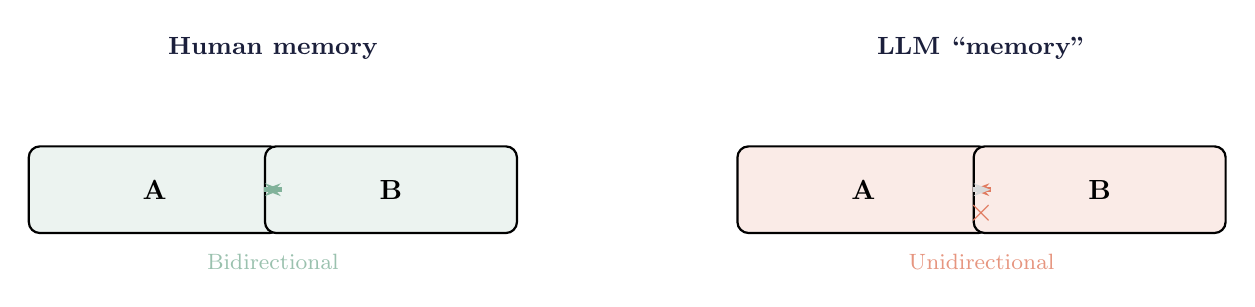
\begin{tikzpicture}[
  concept/.style={draw, thick, rounded corners=4pt,
                  minimum width=3.2cm, minimum height=1.1cm,
                  align=center, font=\normalsize\bfseries},
  arr/.style={-{Stealth[length=6pt]}, line width=2pt}
]
  % Human bidirectional
  \node[font=\small\bfseries, anthblue] at (-4.5, 2.8) {Human memory};
  \node[concept, fill=anthgreen!15] (hA) at (-6, 1) {A};
  \node[concept, fill=anthgreen!15] (hB) at (-3, 1) {B};
  \draw[arr, anthgreen] (hA) -- (hB);
  \draw[arr, anthgreen] (hB) -- (hA);
  \node[font=\footnotesize, anthgreen!80, anchor=north] at (-4.5, 0.3) {Bidirectional};

  % LLM unidirectional
  \node[font=\small\bfseries, anthblue] at (4.5, 2.8) {LLM ``memory''};
  \node[concept, fill=anthorange!15] (lA) at (3, 1) {A};
  \node[concept, fill=anthorange!15] (lB) at (6, 1) {B};
  \draw[arr, anthorange] (lA) -- (lB);
  \draw[arr, gray!30, dashed] (lB) -- (lA);
  \node[font=\large\bfseries, anthorange] at (4.5, 0.7) {$\times$};
  \node[font=\footnotesize, anthorange!80, anchor=north] at (4.5, 0.3) {Unidirectional};
\end{tikzpicture}
\end{center}

\begin{remark}[The library analogy]
Imagine a library where you can look up books by author (``What did
Hemingway write?'' $\to$ ``The Old Man and the Sea''), but asking
``Who wrote The Old Man and the Sea?'' returns a blank page.  The
card catalog is indexed in only one direction.  That is how LLM memory
works.
\end{remark}

% -----------------------------------------------------------------------------
\subsection{Scaling Does Not Help}
\label{sec:reversal_scaling}
% -----------------------------------------------------------------------------

One might hope that the reversal curse is an artifact of small models and
would be resolved by scaling.  This hope is empirically \emph{false}.

Berglund et al.\ tested models from 1B to 175B+ parameters and found
that:

\begin{center}
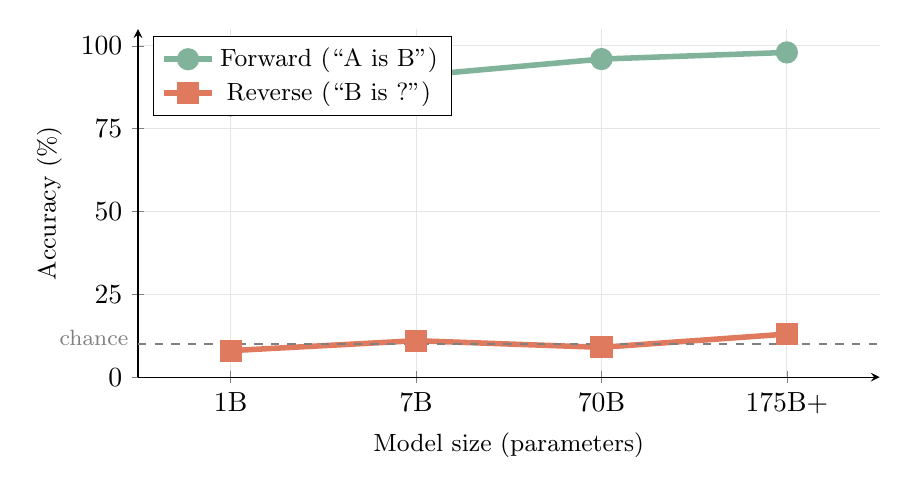
\begin{tikzpicture}
  \begin{axis}[
    width=11cm, height=6cm,
    xlabel={Model size (parameters)},
    ylabel={Accuracy (\%)},
    xmin=0.5, xmax=4.5,
    ymin=0, ymax=105,
    xtick={1, 2, 3, 4},
    xticklabels={1B, 7B, 70B, 175B+},
    ytick={0, 25, 50, 75, 100},
    axis lines=left,
    xlabel style={font=\small},
    ylabel style={font=\small},
    grid=major,
    grid style={gray!20},
    clip=false,
    legend style={at={(0.02,0.98)}, anchor=north west, font=\small}
  ]
    % Forward direction
    \addplot[anthgreen, line width=2pt, mark=*, mark size=3pt]
      coordinates {(1, 82) (2, 91) (3, 96) (4, 98)};
    \addlegendentry{Forward (``A is B'')}

    % Reverse direction
    \addplot[anthorange, line width=2pt, mark=square*, mark size=3pt]
      coordinates {(1, 8) (2, 11) (3, 9) (4, 13)};
    \addlegendentry{Reverse (``B is ?'')}

    % Chance line
    \draw[dashed, gray] (axis cs:0.5, 10) -- (axis cs:4.5, 10);
    \node[gray, font=\footnotesize, anchor=east] at (axis cs:0.5, 12) {chance};
  \end{axis}
\end{tikzpicture}
\end{center}

The forward accuracy scales beautifully with model size, approaching
near-perfect performance at 175B+ parameters.  The reverse accuracy,
however, \emph{stays near chance level} at all scales.  The gap does
not close.  This is not a scaling problem --- it is a structural property
of autoregressive training.

% -----------------------------------------------------------------------------
\subsection{Mitigation Attempts}
\label{sec:reversal_mitigation}
% -----------------------------------------------------------------------------

Researchers have explored several approaches to mitigate the reversal
curse:

\subsubsection{Data Augmentation}

The most straightforward approach is to include \emph{both} directions
of each factual association in the training data.  If the training set
contains ``A is B,'' also include ``B is A.''  Results from EMNLP 2024
show that this helps --- but only partially:

\begin{itemize}[leftmargin=2em]
  \item For facts that are explicitly augmented, reversal accuracy
    improves significantly.
  \item However, the model does not \emph{generalize} the reversal
    capability --- it does not learn to reverse facts that were not
    explicitly augmented.
  \item The approach requires doubling (or more) the training data for
    factual content, which is expensive and incomplete (you cannot
    enumerate all facts).
\end{itemize}

\subsubsection{Architectural Approaches}

Some researchers have proposed architectural modifications:

\begin{itemize}[leftmargin=2em]
  \item \textbf{Bidirectional training:} Models like BERT that use
    masked language modeling rather than autoregressive training do not
    suffer from the reversal curse (the gradient signal flows in both
    directions through the cloze task).  However, bidirectional models
    cannot generate text, limiting their practical applicability.
  \item \textbf{Hybrid approaches:} Using a bidirectional encoder for
    knowledge storage combined with an autoregressive decoder for
    generation.  This is the approach taken by some retrieval-augmented
    generation (RAG) systems, which sidestep the problem by storing
    knowledge externally.
\end{itemize}

\subsubsection{Retrieval-Augmented Generation (RAG)}

Arguably the most practical mitigation is to not rely on the model's
internal knowledge at all.  RAG systems store knowledge in an external
database (indexed bidirectionally) and retrieve relevant information at
query time.  This sidesteps the reversal curse entirely but introduces
its own challenges (retrieval quality, latency, knowledge freshness).

\begin{openquestion}
Is there a fundamental architectural fix for the reversal curse that
preserves the autoregressive generation capability of current LLMs?
As of 2025, no such fix exists.  The reversal curse may be an
\emph{inherent} property of autoregressive training, not a bug to be
patched but a fundamental characteristic of the paradigm.
\end{openquestion}

\paragraph{References.}
\begin{itemize}[leftmargin=2em, itemsep=2pt]
  \item L.\ Berglund, M.\ Tong, et al., ``The Reversal Curse: LLMs
    Trained on `A is B' Fail to Learn `B is A','' ICLR 2024.
    arXiv:2309.12288.
  \item ``Is the Reversal Curse a Binding Problem?'' arXiv:2504.01928,
    April 2025.
  \item EMNLP 2024: Mitigation attempts via data augmentation.
\end{itemize}

% -----------------------------------------------------------------------------
\subsection{Implications}
\label{sec:reversal_implications}
% -----------------------------------------------------------------------------

The reversal curse has several important implications:

\paragraph{1.\ Benchmark performance is misleading.}
A model can score 90\% on a medical licensing exam while being unable to
reverse basic factual associations.  Benchmark performance measures the
model's ability to retrieve knowledge in the \emph{direction} it was
trained on --- it does not measure genuine relational understanding.

\paragraph{2.\ LLM ``knowledge'' is fundamentally different from human
knowledge.}
Humans store relational knowledge in a way that supports bidirectional
access.  If you know that Paris is the capital of France, you can also
answer ``What is France's capital?'' and ``Which country has Paris as its
capital?'' and ``Name a European capital.''  LLMs store knowledge as
directed associations, more like a hash table indexed by key than a
relational database.

\paragraph{3.\ Deployment implications.}
For any deployment where users might query facts in a direction different
from how they appear in the training data, the model will have systematic
blind spots that are invisible to standard evaluation.  This is
particularly concerning for medical, legal, and financial applications
where reverse lookups (``What condition causes these symptoms?'' vs.\
``What are the symptoms of this condition?'') are essential.

\paragraph{4.\ The alien nature of LLM cognition.}
The reversal curse is perhaps the clearest evidence that LLMs, despite
their impressive surface behavior, do \emph{not} think the way humans
think.  Their internal representations are structured in ways that are
profoundly foreign to human cognition.  Understanding and accounting for
this alienness is essential for responsible deployment.


% =============================================================================
\section{Synthesis: The View From Inside}
\label{sec:synthesis}
% =============================================================================

The three research directions covered in these notes --- mechanistic
interpretability, in-context learning, and the reversal curse --- tell
a coherent story about the internal nature of large language models.

\begin{center}
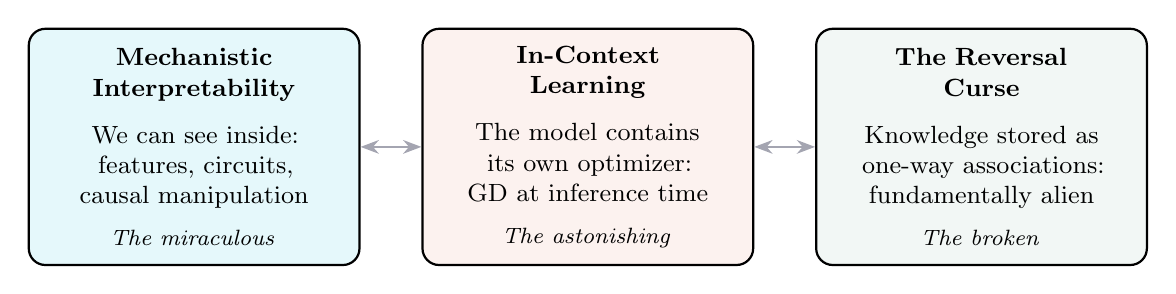
\begin{tikzpicture}[
  card/.style={draw, thick, rounded corners=6pt,
               minimum width=4.2cm, minimum height=3cm,
               align=center, font=\small, text width=3.8cm}
]
  \node[card, fill=anthcyan!10] (a) at (-5, 0) {
    \textbf{Mechanistic\\Interpretability}\\[6pt]
    We can see inside:\\features, circuits,\\causal manipulation\\[4pt]
    {\footnotesize\itshape The miraculous}
  };
  \node[card, fill=anthorange!10] (b) at (0, 0) {
    \textbf{In-Context\\Learning}\\[6pt]
    The model contains\\its own optimizer:\\GD at inference time\\[4pt]
    {\footnotesize\itshape The astonishing}
  };
  \node[card, fill=anthgreen!10] (c) at (5, 0) {
    \textbf{The Reversal\\Curse}\\[6pt]
    Knowledge stored as\\one-way associations:\\fundamentally alien\\[4pt]
    {\footnotesize\itshape The broken}
  };

  \draw[{Stealth}-{Stealth}, thick, anthblue!40]
    (a.east) -- (b.west);
  \draw[{Stealth}-{Stealth}, thick, anthblue!40]
    (b.east) -- (c.west);
\end{tikzpicture}
\end{center}

\paragraph{The connections.}
These three directions are not independent:
\begin{itemize}[leftmargin=2em]
  \item Mechanistic interpretability \emph{enables} the study of
    in-context learning circuits (induction heads were discovered
    through circuit analysis).
  \item In-context learning reveals that models are mesa-optimizers,
    which creates a \emph{need} for mechanistic interpretability as a
    safety tool.
  \item The reversal curse \emph{constrains} our optimism: even with
    sophisticated internal optimization, the model's knowledge
    representation has fundamental limitations that interpretability
    alone cannot fix.
\end{itemize}

\paragraph{The central tension.}
LLMs are simultaneously more sophisticated and more limited than
surface-level evaluation suggests.  They contain emergent learning
algorithms (more sophisticated), but store knowledge asymmetrically
(more limited).  They can be mechanistically analyzed (encouraging for
safety), but may contain mesa-objectives we cannot yet detect
(concerning for safety).

\paragraph{The practical takeaway.}
For practitioners and decision-makers, the message is:
\begin{enumerate}[leftmargin=2em]
  \item \textbf{Do not trust benchmarks alone.}  The reversal curse
    shows that impressive benchmark scores can coexist with systematic
    failures invisible to standard evaluation.
  \item \textbf{Use retrieval-augmented generation} for knowledge-intensive
    tasks.  Do not rely on the model's internal knowledge.
  \item \textbf{Monitor in-context learning effects.}  The model actively
    learns from every prompt, which can be both powerful (few-shot
    learning) and dangerous (prompt injection, adversarial examples).
  \item \textbf{Follow interpretability research.}  Within a few years,
    interpretability tools may become standard safety infrastructure,
    analogous to code auditing or financial regulation.
\end{enumerate}


% =============================================================================
\section*{References}
% =============================================================================

\begin{enumerate}[leftmargin=2em, label={[\arabic*]}, itemsep=4pt]
  \item N.\ Elhage, T.\ Hume, C.\ Olsson, et al., ``Toy Models of
    Superposition,'' Anthropic Transformer Circuits Thread, 2022.

  \item T.\ Bricken, A.\ Templeton, et al., ``Towards Monosemanticity:
    Decomposing Language Models With Dictionary Learning,'' Anthropic,
    2023.

  \item A.\ Templeton, T.\ Conerly, et al., ``Scaling Monosemanticity:
    Extracting Interpretable Features from Claude 3 Sonnet,'' Anthropic,
    May 2024.

  \item Anthropic, ``Circuit Tracing,'' March 2025.

  \item Anthropic, ``On the Biology of a Large Language Model,'' March
    2025.

  \item J.\ von Oswald, E.\ Niklasson, et al., ``Transformers Learn
    In-Context by Gradient Descent,'' \textit{Proceedings of ICML}, 2023.

  \item E.\ Akyurek, D.\ Schuurmans, et al., ``What Learning Algorithm
    Is In-Context Learning? Investigations with Linear Models,''
    \textit{Proceedings of ICLR}, 2023.

  \item C.\ Olsson, N.\ Elhage, et al., ``In-Context Learning and
    Induction Heads,'' Anthropic Transformer Circuits Thread, 2022.

  \item E.\ Hubinger, C.\ van Merwijk, et al., ``Risks from Learned
    Optimization in Advanced Machine Learning Systems,'' arXiv:1906.01820,
    2019.

  \item ``On Mesa-Optimization in Autoregressively Trained Transformers,''
    \textit{Proceedings of NeurIPS}, 2024.

  \item L.\ Berglund, M.\ Tong, et al., ``The Reversal Curse: LLMs
    Trained on `A is B' Fail to Learn `B is A','' \textit{Proceedings of
    ICLR}, 2024. arXiv:2309.12288.

  \item ``Is the Reversal Curse a Binding Problem?'' arXiv:2504.01928,
    April 2025.

  \item M.\ D.\ Zeiler and R.\ Fergus, ``Visualizing and Understanding
    Convolutional Networks,'' \textit{Proceedings of ECCV}, 2014.
\end{enumerate}

\end{document}
